\chapter{Simulación de tráfico}
\label{ch:sota-traffic-simulation}

\marginnote{
	A lo largo del capítulo, se utilizarán indistintamente los términos \Acrfull{dvu}\index{driver-vehicle unit}, conductor y vehículo para referirse al mismo concepto. En caso de no ser así, se indicará de manera explícita.
}

El tráfico es un sistema de comportamiento caótico que hace muy difícil la tarea de extraer de modelos de funcionamiento. Por un lado, la cantidad de variables existentes es muy numerosa y en muchos casos con relaciones no detectables a primera vista. Por otro lado, es un sistema que funciona en el mundo real, es decir, donde las mediciones en unos casos afectan a los resultados y en otros, directamente no se pueden realizar, ya sea por regulaciones vigentes o por imposibilidad física.

Los simuladores de tráfico son herramientas de software que, usando diferentes modelos para representar sus componentes, describen el tráfico como sistema, permitiendo, entre otros:

\begin{itemize}
	\item Extracción de resultados y conclusiones de escenarios de tráfico determinados.
	\item Implementación de técnicas determinadas en tráfico simulado para su evaluación sin necesidad de alterar el tráfico real.
	\item Introducción de modificaciones en puntos determinados (e.g. espaciales o temporales) de un escenario conocido para estudiar la divergencia en la evolución del tráfico.
\end{itemize}

El objetivo principal de un simulador de tráfico es el de hacer que sus modelos se parezcan lo máximo posible a la realidad. En este capítulo vamos a ver cuál es la realidad actual de este tipo de simuladores, cuáles son sus diferentes tipologías y formas de modelar los diferentes aspectos del tráfico y, posteriormente, qué simulador de los disponibles en el mercado es el idóneo para nuestro trabajo.

Limitaremos nuestro estudio a los simuladores de \Acrfullpl{dvu}\index{driver-vehicle unit}, obviando otros tipos de simulación de tráfico que nada tienen que ver con esta temática, como por ejemplo los orientados a la evaluación de sistemas de señalización inteligentes (e.g.~\cite{jin2016evaluation}), a la estimación de emisiones (e.g.~\cite{quaassdorff2016microscale}) o los de carreras (e.g. \cite{Wymann2013}).

\section{Clasificación de simuladores de tráfico}

Los aspectos simulables y medibles del problema del tráfico son muy diversos (Figura~\ref{fig:how-to-simulate-traffic}), dependiendo sobre todo:

\begin{figure}
	\centering
	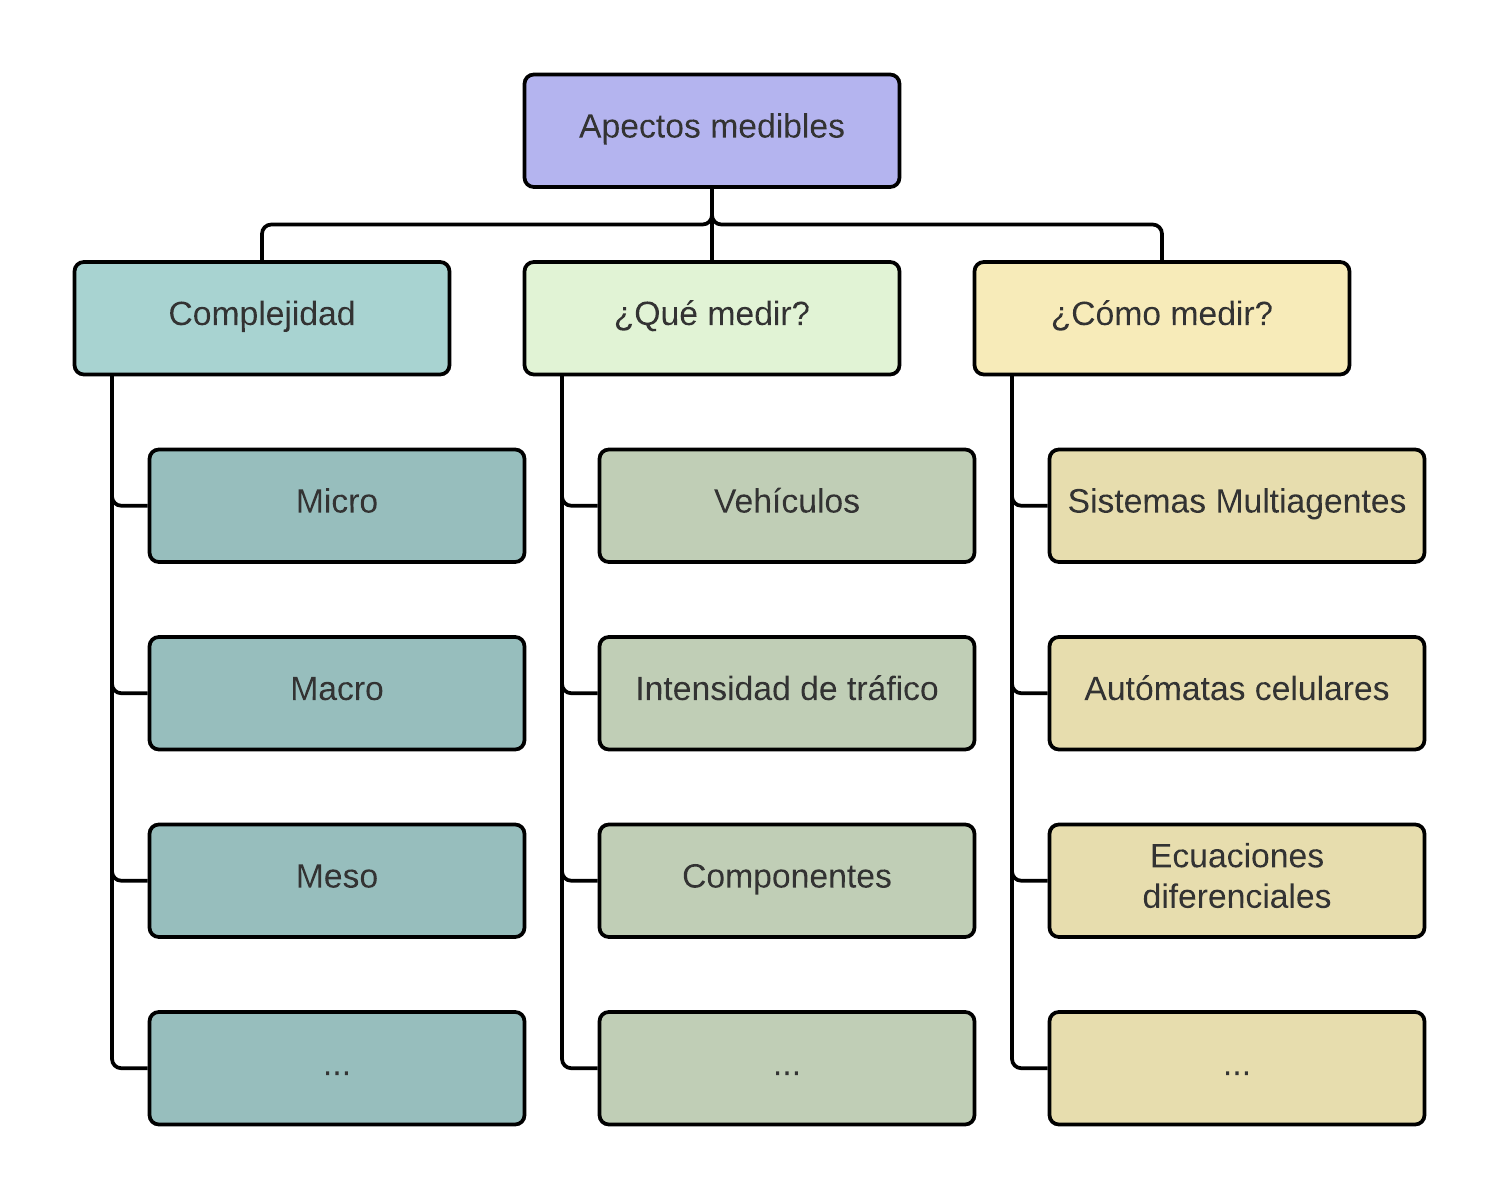
\includegraphics{how-to-simulate-traffic}
	\caption[Aspectos medibles del tráfico]{Aspectos medibles del tráfico. Son muy diversos, y dependen del nivel de granularidad (complejidad) al que se quiere llegar, de qué queremos medir y de cómo lo queremos hacer.}
	\label{fig:how-to-simulate-traffic}
\end{figure}

\begin{itemize}
	\item Del nivel de \textbf{complejidad} del tráfico (e.g. modelar una vía por la que circula un centenar de coches no es lo mismo que modelar una ciudad por la que circulan cientos de miles).
	\item De \textbf{qué} queremos medir (e.g. evaluar a un conductor en una situación determinada o evaluar la evolución del flujo de tráfico en un cuello de botella causado por un accidente).
	\item De \textbf{cómo} (e.g. un \acrlongsp{ca}\index{autómata celular} se modela de forma diferente a un modelo lineal de vías o carriles).
\end{itemize}

El resto de la sección ofrece una visión de las principales categorías existentes para clasificar a los simuladores de tráfico.

\subsection{Tipos de simulador en función de la complejidad}

La complejidad en una simulación se refiere al nivel de detalle que queremos alcanzar durante la ejecución de la misma y/o en sus resultados. Es evidente que según aumentamos el detalle en la simulación aumenta la cantidad de cálculo. Por ejemplo, si queremos modelar el comportamiento de $10$ billones de canicas cayendo por un tubo es considerablemente más eficiente modelarlas como un fluido con una serie de parámetros que como una colección de elementos individuales, cada uno con sus propiedades (e.g. masa, aceleración, \ldots) e interaccionando entre sí.

El caso de los simuladores de tráfico es similar. En éstos existe un amplio intervalo de granularidades, desde por ejemplo el flujo de entrada en una autovía hasta el consumo de carburante de un vehículo en ciudad. Lo más común es clasificar los simuladores dentro de dos grandes grupos (Figura~\ref{fig:granularities-in-traffic-simulation}):

\begin{figure}
	\centering
	\subfloat[Macroscópico]{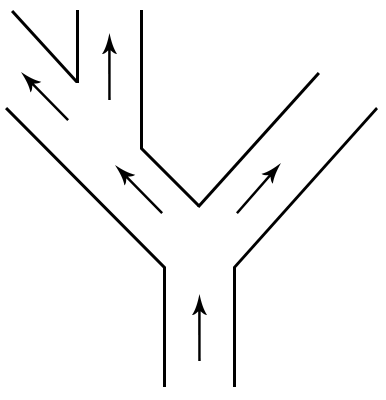
\includegraphics[height=5cm]{macroscopic}}\qquad
	\subfloat[Microscópico]{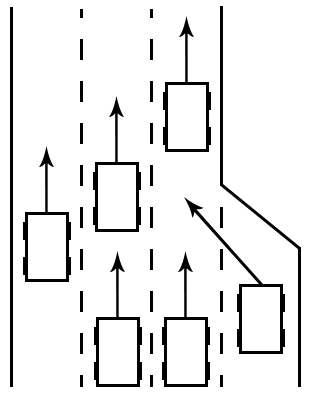
\includegraphics[height=5cm]{microscopic}}
	\caption[Clasificación de simuladores según granularidad]{Clasificación clásica de simuladores en función de la granularidad (complejidad) de la simulación. En la imagen de la izquierda se muestra un ejemplo clásico de macrosimulador donde el tráfico se modela como un flujo a través de las vías. En la de la derecha, se ilustra un modelo clásico de micro-simulación donde cada elemento (en este caso vehículos) circula por un carril de la vía.}
	\label{fig:granularities-in-traffic-simulation}
\end{figure}

\begin{itemize}
	\item \textbf{Microsimulación} o simulación de tipo \textbf{micro}. Su objetivo es estudiar, desde un punto de vista de granularidad fina (e.g. vehículos o peatones), las micropropiedades del flujo de tráfico como, por ejemplo, los cambios de carril, las aproximaciones a vehículos delanteros o los adelantamientos, para evaluar su comportamiento. Sus dos principales ventajas son la posibilidad de estudiar el tráfico como un todo a partir de sus elementos más simples (ofreciendo una representación más fiel de éste) y la posibilidad de estudiar cada elemento por separado. Sin embargo, su principal desventaja es que cada elemento de la simulación requiere de cómputo independiente y por tanto simulaciones con alto contenido de elementos pueden llegar a ser inviables\sidenote{
		Existen técnicas de computación distribuida que superan ampliamente los límites impuestos por la computación en un único nodo. Un ejemplo relativamente reciente es el simulador de IBM \textit{Megaffic}. Éste implementa un modelo de granularidad micro donde cada elemento es un agente independiente (i.e. \acrlongplsp{mas}\index{sistemas multiagente}) usando para ello entornos con cientos de núcleos de proceso que proveen de capacidad suficiente para modelar ciudades enteras como Tokio (ver~\cite{Osogami2012} y~\cite{Suzumura2012}).
	}.
	\item \textbf{Macrosimulación} o simulación de tipo \textbf{macro}. Este tipo de modelos centran su esfuerzo en estudiar el flujo de tráfico como un todo (generalmente como fluido), explorando sus macropropiedades (e.g. evolución del tráfico, efectos onda, velocidad media o flujo en vías). Su ventaja principal es que a nivel macroscópico permiten estudiar propiedades que a nivel microscópico requerirían una cantidad ingente de recursos. Sin embargo, con este modelo es imposible obtener información precisa de un elemento en particular del tráfico.
\end{itemize}

Aunque ésta es la categorización típica de modelos, en la literatura aparecen otros tipos de modelo con granularidades que pueden considerarse no pertenecientes a ninguno de estos dos conjuntos. Éste es el caso de los simuladores de tipo \textbf{submicro} y de tipo \textbf{meso}.

Los \textbf{submicro-modelos} (también denominados como \textit{nano-modelos} en algunos trabajos) especifican granularidades por debajo del nivel de \enquote{vehículo} o \enquote{peatón}. Por ejemplo, en (\cite{Minderhoud1999}) trabaja a nivel de funcionamiento del control de crucero inteligente de un vehículo en función del entorno del vehículo.

Por otro lado los \textbf{meso-simuladores} nacen para amortiguar los problemas inherentes a la complejidad en los micro-modelos y a la falta de resolución en los macro-modelos. Este tipo de simulador mantiene la representación de vehículo como unidad básica de tráfico, pero agrega dinámicas de tráfico que, de otro modo, aumentarían el consumo de recursos sin aportar información relevante sobre la tarea en la que trabajan.b Los trabajos en la línea de meso-modelos no se basan en una simulación completa a nivel meso, sino que trabajan desde una perspectiva híbrida, como por ejemplo el de \cite{munoz2001integrated} donde utilizan una aproximación meso para reducir el coste computacional de simulaciones micro a una escala muy grande, o el de \cite{casas2011need}, un estudio similar específico para \gls{aimsun}.

Dado que el objetivo de la tesis es la evaluación de modelos de comportamiento de conductores concretos, nos ceñiremos al uso de simuladores que modelen un nivel de granularidad \textbf{micro}.

\subsection{Tipos de simulador en función del espacio y el tiempo}

Existen otras dos formas de clasificar los simuladores en función de cómo evolucionan en la simulación las dimensiones \textbf{espacio} y  \textbf{tiempo}. Sin embargo, aunque \textit{complejidad}, \textit{espacio} y \textit{tiempo} son dimensiones diferentes a la hora de clasificar, el tipo de simulador según una de ellas tiende a determinar en gran medida los tipos en las demás.

En el caso de la dimensión \textbf{espacio}, la clasificación diferencia las simulaciones que se mueven por un espacio discreto o por uno continuo:

\begin{itemize}
	\item Espacio \textbf{discreto}. Simulación donde el espacio está dividido en celdas que (normalmente) sólo pueden estar ocupadas por un elemento en un momento determinado. Este es el caso, por ejemplo, de los simuladores basados en \acrlongplsp{ca}\index{autómata celular} (Figura~\ref{fig:cellular-automata-based-sim}).

	\begin{figure}
		\centering
		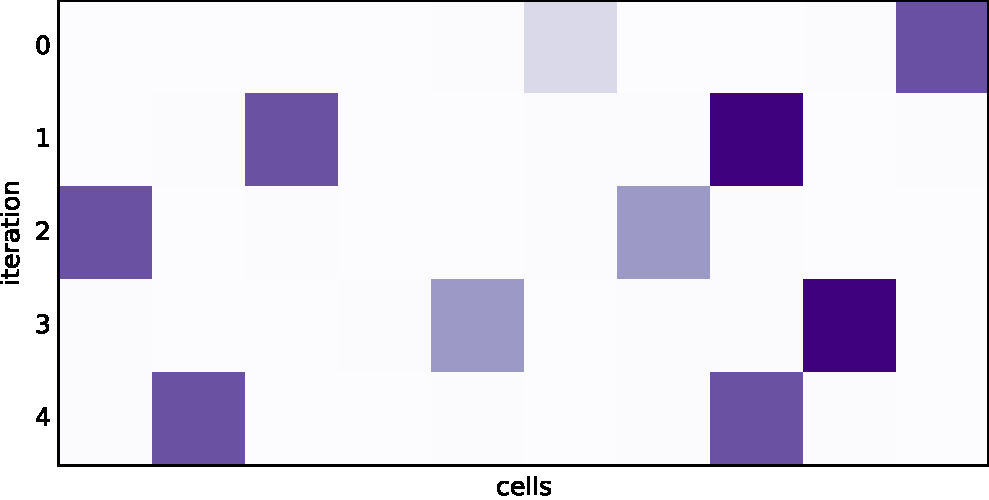
\includegraphics[width=10cm]{cellular-automata-based-sim}
		\caption[Ejemplo de simulador basado en \acrlongsp{ca}]{Ejemplo de simulador basado en \acrlongsp{ca}. El espacio se divide en celdas que pueden estar vacías u ocupadas por un vehículo a una velocidad (más oscuro implica más lento). Concretamente muestra la evolución a lo largo del tiempo del movimiento de un modelo de \textit{\gls{car-following}} de $2$ vehículos donde en eje $x$ representa la posición en la vía y el eje $y$ el momento temporal (iteración) de la vía.}
		\label{fig:cellular-automata-based-sim}
	\end{figure}

	\item Espacio \textbf{continuo}. Simulación que transcurre en una secuencia infinita de puntos en el espacio. Es el caso por ejemplo de los simuladores basados en modelos lineales (Figura~\ref{fig:car-following-based-sim}).
	
	
	\begin{figure}
		\centering
		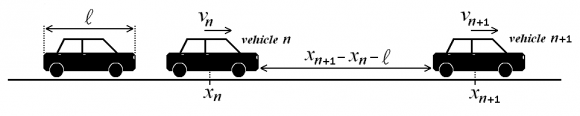
\includegraphics{car-following-based-sim}
		\caption[Ejemplo de modelo lineal en un espacio continuo]{Ejemplo de un modelo lineal en un espacio continuo. La posición del vehículo es un valor $x \in \mathbb{R}$. Este ejemplo muestra un modelo de \textit{\gls{car-following}} donde el comportamiento de la aceleración del vehículo es determinado por la distancia al coche siguiente. Fuente:~\cite{Tordeux2011}.}
		\label{fig:car-following-based-sim}
	\end{figure}
	
\end{itemize}

En el caso de la dimensión \textbf{tiempo}, la división se realiza en los mismos términos que en los del espacio:

\begin{itemize}
	\item Tiempo \textbf{discreto}. También denominada \textit{simulación de eventos discretos}, divide el tiempo en intervalos discretos, generalmente de longitud fija durante toda la simulación. Los simuladores basados en \acrlongplsp{ca}\index{autómata celular} son típicamente discretos, ya que cada posición en el espacio se va calculando para cada intervalo discreto de tiempo (Figuras~\ref{fig:cellular-automata-based-sim} y~\ref{fig:nagel-schreck}).
	
	\begin{figure}
		\centering
		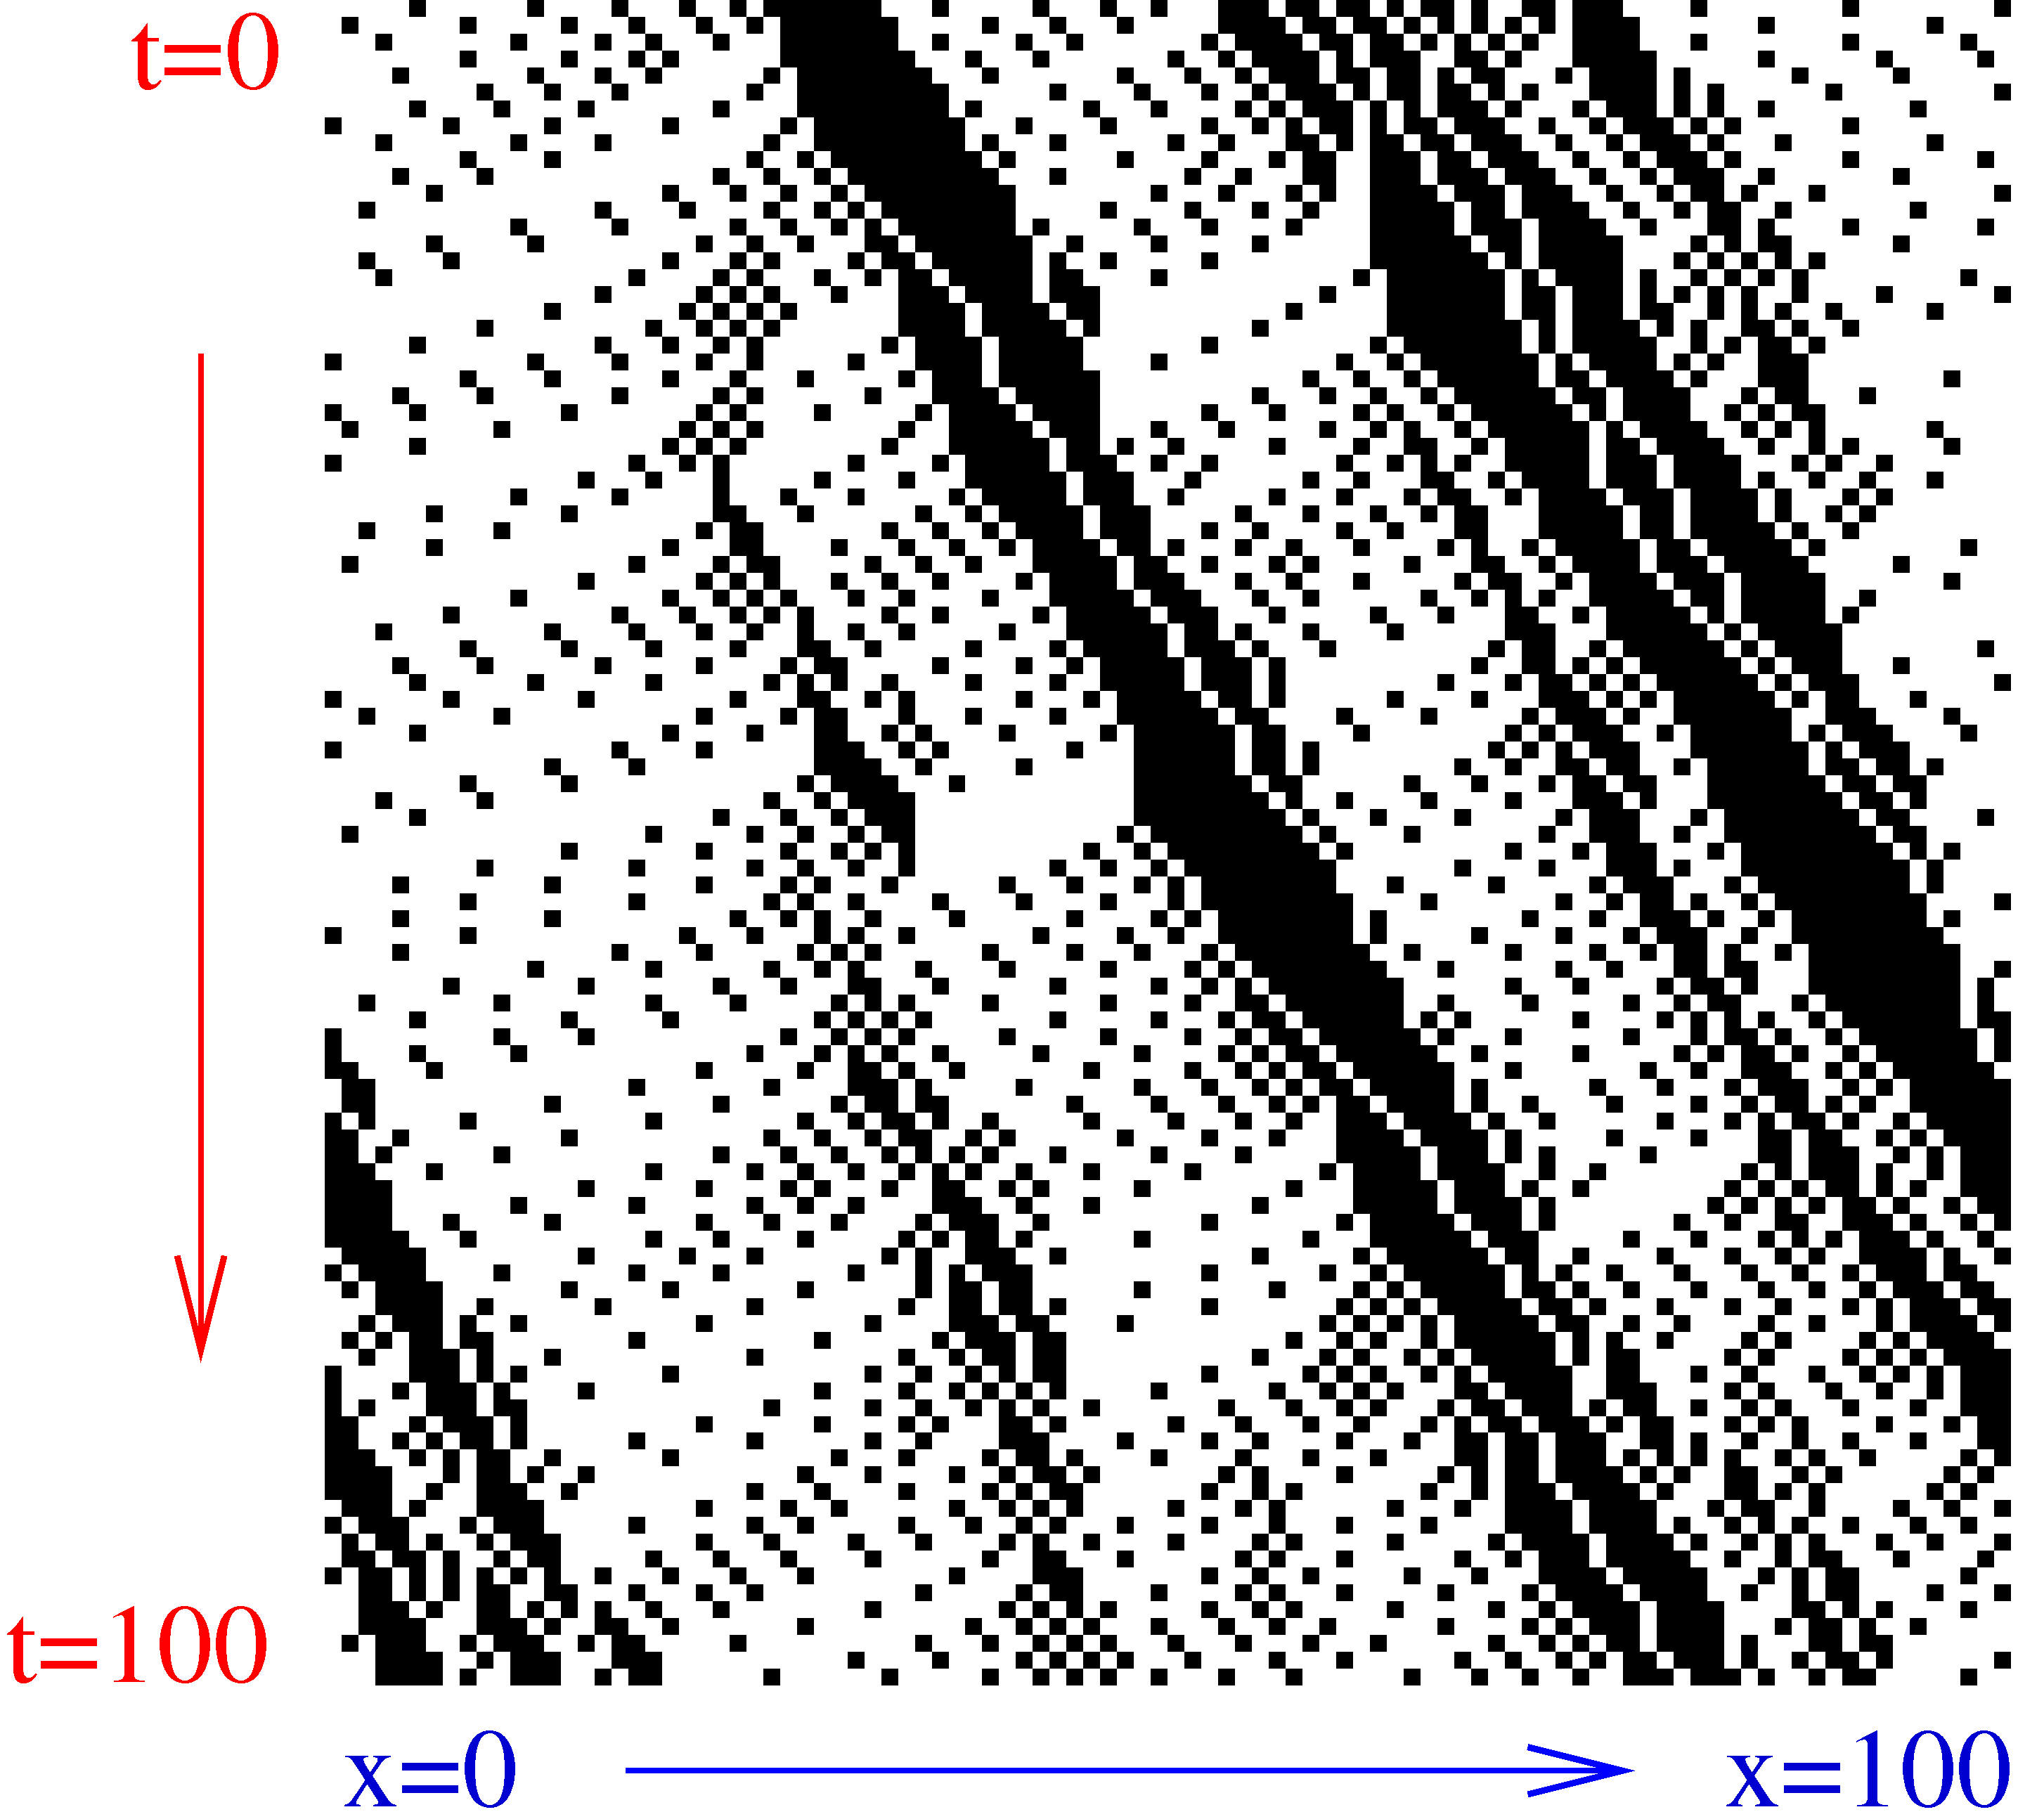
\includegraphics{nagel-schreck}
		\caption[Ejemplo de efecto de ondas de choque en simulación de tipo Nagel-Scherckenberg]{Ejemplo de efecto de ondas de choque en simulación de tipo Nagel-Scherckenberg. La longitud de la autopista es de $250$ celdas, su densidad de ocupación de $50$ coches en la vía, la velocidad máxima $5 c/\Delta t$ y la probabilidad de frenada es de $p = 0.5$. Se puede observar en la figura cómo se desplazan las \enquote{olas} del atasco a lo largo de las $100$ iteraciones.}
		\label{fig:nagel-schreck}
	\end{figure}
	
	\item Tiempo \textbf{continuo}. En estos simuladores el tiempo es un factor más para un modelo de ecuaciones diferenciales. La Figura~\ref{fig:car-following-based-sim} ilustra un modelo de \textit{\gls{car-following}\index{car-following}} que puede implementarse en una simulación de tiempo continuo si la aceleración viene determinada por un modelo que entre otros factores incluye el tiempo.
\end{itemize}

En nuestro caso, queremos conocer la situación exacta del vehículo en lugar de una situación aproximada en un dominio espacial discreto. También realizaremos la recolección de datos en intervalos cuantificables de tiempo, los cuales serán usados para modelar los comportamientos de los conductores y para contrastar los resultados.

Nuestro estudio se ceñirá, por tanto, hacia el trabajo sobre micro-simuladores de \textbf{espacio continuo} y \textbf{eventos discretos}.

\section{Modelos de micro-simulación}

Los simuladores que se basan en un modelo de granularidad micro están en su mayoría implementados en dos tipos de paradigma: \acrlongplsp{ca}\index{autómata celular} y \acrlongplsp{mas}\index{sistemas multiagente}.

Existe un tercer punto de vista a la hora de implementar este tipo de modelos, que es el de los sistemas de partículas. Sin embargo, su ámbito de aplicación es el mismo que el del punto de vista macroscópico, esto es, usar sistemas de partículas para el análisis del tráfico como fluido. Por tanto, el resto de la sección describirá los dos tipos principales sin tener en cuenta éste último.

\subsection{Micro-simulación basada en \acrlongplsp{ca}\index{autómata celular}}

Un \Acrfull{ca}\index{autómata celular} es una colección ordenada de celdas (\textit{células}) en un espacio $n$-dimensional que parcelan el universo de estudio. Cada una de ellas se encuentra en un estado (e.g. contiene un valor numérico), y el estado de toda la malla se actualiza de manera síncrona\sidenote{
	Existen arquitecturas diseñadas para operar de esta manera, esto es, arquitecturas basadas en \gls{ca}\index{autómata celular} (e.g.~\cite{Margolus1993}). En ellas, cada ciclo de reloj actualiza todas las celdas de memoria del autómata. Éstas arquitecturas se suelen usar para la implementación de modelos físicos superando en varios órdenes de magnitud la capacidad computacional de las arquitecturas tradicionales.
} (i.e., todas a la vez) en intervalos regulares de tiempo denominados \textit{ciclos}. El cambio de estado de cada célula depende de los valores de las células vecinas y del mismo algoritmo de modificación al que responden todas y cada una de las células.

Por su naturaleza, los modelos de de micro-simulación basados en este paradigma se clasifican como simuladores de tiempo y espacio discreto, y son usados por su facilidad de implementación y porque son fácilmente paralelizables.

El modelo clásico de esta aproximación es el propuesto por Nagel-Scherckenberg en su artículo \textit{A cellular automaton model for freeway traffic} \cite{Nagel1992}, un modelo teórico creado para la simulación de tráfico en autopistas. La Figura~\ref{fig:nagel-schreck} muestra la evolución del tráfico en una autopista a lo largo del tiempo en una implementación basada en este paradigma.

\marginnote{
	\textbf{El modelo Nagel-Scherckenberg} es un \glsentrylongsp{ca}\index{autómata celular} que basa su funcionamiento en los siguientes aspectos:
	
	\begin{itemize}
		\item La vía está divida en celdas de longitud $7,5m$. La razón de este valor es que ésta es la distancia media entre los parachoques traseros de dos coches consecutivos en un atasco.
		\item La celda puede tener dos estados, vacía o con un vehículo a velocidad $v = \{0, \ldots, v_{max}\} \in \mathbb{N}$. La unidad de medida es $c/\Delta t$ (celdas por unidad de tiempo).
		\item $\Delta t$ queda establecido en \SI{1}{\second}, considerado el tiempo medio de reacción de un conductor ante una eventualidad. Esto hace, por ejemplo, que una velocidad de $6 c/\Delta t$ sea $45 m/s$ ($162 km/h$).
		\item En cada ciclo y para cada vehículo, se realizan tres acciones de manera consecutiva: (i) acelerar una unidad si no está a la máxima velocidad o frenar si se ve obligado, (ii) freno aleatorio (la velocidad se reduce en una unidad hasta un mínimo de $v = 1 c/\Delta t$ con una probabilidad de $p = 0.5$) y (iii) reposicionamiento.
	\end{itemize}
}

En general los modelos de la literatura suelen ser una variación del de Nagel-Scherckenberg con modificaciones para estudiar aspectos concretos de modelos de tráfico o para dotarle de un mayor realismo. Algunos ejemplos de estas variaciones son la modificación del paso de \textit{aleatorización} (e.g. \cite{Barlovic1998}), reglas para determinar niveles de molestia a vehículos vecinos (\cite{Wagner1997}), celdas más pequeñas (e.g. \cite{Krauss1997}) para comprobar la metaestabilidad del flujo de tráfico, o modelos y reglas para cambio de carril\index{lane-change} en vías de dos carriles (\cite{Brilon1999, Nagel1998}).

Los modelos basados en \acrlongplsp{ca}\index{autómata celular} no son suficientemente realistas desde un punto de vista microscópico. Por poner un ejemplo, en una situación típica de un modelo Nagel-Scherckenberg, los vehículos realizan aleatoriamente aceleraciones y deceleraciones de \SI{27}{\kilo\meter\per\square\hour}. Es más, en una situación favorable, cualquier vehículo puede realizar una aceleración de \SI{0}{\kilo\meter\per\hour} a \SI{162}{\kilo\meter\per\hour} en tan sólo \SI{6}{\second} segundos. Por tanto, no ofrecen una visión demasiado realista ni fiable en caso de querer realizar estudios muy detallados de tráfico.

\subsection{Micro-simulación basada en \acrlongplsp{mas}\index{sistemas multiagente}}

Por otro lado, en un \acrlongplsp{mas}\index{sistemas multiagente} cada uno de los agentes tiene su propia entidad dentro del sistema. Esto es, perciben tanto el entorno como al resto de agentes y actúan de acuerdo a lo percibido y a su comportamiento. Basarse no sólo en las magnitudes físicas del resto de vehículos (e.g. distancia, aceleración, \ldots) sino también en un comportamiento de conducción ofrece un interesante campo de estudio a nivel cognitivo. Se habla más en detalle sobre los \acrlongplsp{mas}\index{sistemas multiagente} en el capítulo \nameref{ch:sota-ci} y sobre los comportamientos concretos de agentes de interés para esta tesis en el capítulo~\ref{ch:sota-behavior-models}. Por ello, este apartado únicamente hará una pequeña introducción a estudios existentes y aplicaciones de simuladores basados en este modelo.

A diferencia de los \acrlongplsp{ca}\index{autómata celular}, los \acrlongplsp{mas}\index{sistemas multiagente} pueden emplazarse en un entorno virtual que represente un espacio continuo y no discreto. Esto permite modelar con mayor fidelidad magnitudes físicas asociadas a cada agente (e.g. posición y velocidades actuales, dimensiones del vehículo, masa, velocidad máxima permitida, \ldots). Sin embargo, aun así no es una propiedad inherente de éstos. No existe ninguna limitación en cuanto a la representación del espacio y es perfectamente posible representar un modelo basado en \acrlongplsp{ca}\index{autómata celular} usando para ello \acrlongplsp{mas}\index{sistemas multiagente}.

Cada uno de los agentes es independiente del resto, y una consecuencia directa es que el comportamiento de cada individuo permite evaluar comportamientos grupales complejos, como el descrito en la Figura~\ref{fig:autonomous-vehicles-at-intersections}. Esta independencia da la posibilidad de tener todos los agentes diferentes entre sí, ofreciendo la ventaja de permitir experimentar con diferentes perfiles de conducción (e.g. un perfil agresivo en un flujo de tráfico dominado por conductores tranquilos).

\begin{figure}
	\centering
	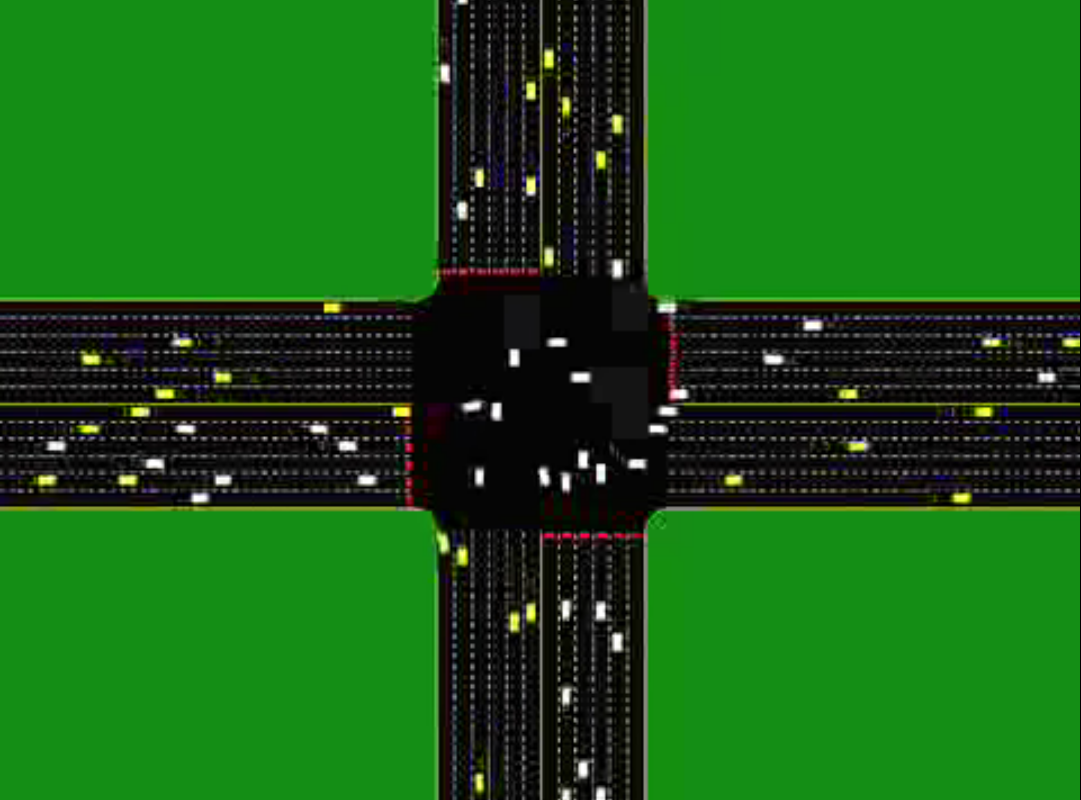
\includegraphics[width=10cm, height=4.9cm]{autonomous-vehicles-at-intersections}
	\caption[Simulación de comportamiento en intersección basada en un \acrlongsp{mas}]{Simulación de comportamiento en intersección basada en un \acrlongsp{mas}. En ésta, cada uno de los vehículos incorpora un controlador para hacerlo autónomo. Modelar este caso de estudio con una arquitectura basada en \acrlongplsp{mas} permite centrarse en el diseño del agente en concreto (i.e. el controlador de conducción del vehículo) y estudiar el comportamiento emergente surgido de la interacción de todos los agentes. Fuente: Proyecto AIM (\url{http://www.cs.utexas.edu/~aim/}).}
	\label{fig:autonomous-vehicles-at-intersections}
\end{figure}

Esto es debido a que en un \acrlongsp{mas}\index{sistemas multiagente} cada agente es una parte del sistema y las decisiones de cómo se ha de comportar las toma él mismo. Desde el punto de vista de un \acrlongsp{ca}\index{autómata celular}, el comportamiento existe en cada celda, sin dar control al contenido o estado de cada celda.

En general los estudios basados en este modelo suelen seguir el patrón $1 \text{ \gls{dvu}\index{driver-vehicle unit}} \equiv 1 \text{ agente}$, dando así una enorme cantidad de posibilidades a experimentar. Por ejemplo en \cite{Das} se hace uso de \acrlongplsp{fcs}\index{sistema de control borroso} para decidir cómo comportarse en la vía mientras que en \cite{Ehlert2001} se hace uso de un patrón reactivo. Otros, como \cite{Dia2002} o \cite{Balmer} hacen uso de encuestas o censos para establecer las propiedades y calibrar los parámetros de diferentes tipos de agentes.

Los estudios en materia de simuladores de tráfico con \glsentrylongsp{mas}\index{sistemas multiagente} no se limitan a vehículos, sino que se usan también en otras áreas como el control de luces de tráfico o agentes para peatones entre otros. Por ejemplo el estudio presentado en \cite{Clymer2002}, los agentes del sistema son las señales de tráfico luminosas y no los vehículos, y el objetivo es adaptar la señalización en una red de carreteras para minimizar al máximo el tiempo de espera por parte de los vehículos en las intersecciones gestionadas por las señales. Otro ejemplo es el propuesto en \cite{Galis2000}, donde los agentes, en lugar de ser los vehículos son los tramos de las carreteras; en él, los vehículos poseen comportamiento, pero lo reciben del agente que les guía de acuerdo a la zona en la que se encuentran. Esto tiene la ventaja de que el paso de información a vehículos dentro de la misma zona se realiza mucho más rápido en un entorno distribuido.

En los últimos años, otro concepto que está en auge es el de las redes intervehiculares e intravehículares, \gls{v2v}\index{v2v} y \gls{v2i}\index{v2i}. El modelo de \acrlongplsp{mas}\index{sistemas multiagente} permite la implementación rápida de diferentes políticas y protocolos de comunicación via sensores y actuadores para estudiar estos tipos de redes de comunicación (Figura~\ref{fig:cooperative-traffic-movsim}).

\begin{figure}
	\centering
	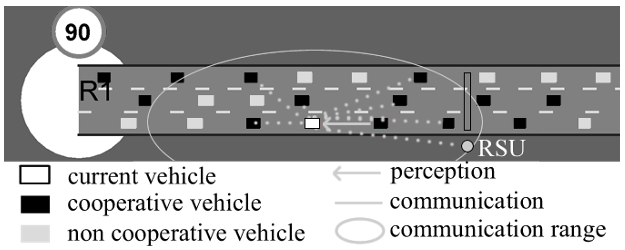
\includegraphics{cooperative-traffic-movsim}
	\caption[Captura de pantalla del simulador \gls{movsim}]{Captura de pantalla del simulador \gls{movsim}. Este simulador implementa un modelo multiagente donde los vehículos incorporan sistemas de comunicación vehicular. El estudio se centra en el uso de la comunicación entre vehículos para el acoplamiento dinámico de vehículos en sus respectivos carriles. Fuente: \cite{Gu2015}.}
	\label{fig:cooperative-traffic-movsim}
\end{figure}

Estudios como por ejemplo \cite{Shiose2001} o \cite{Galis2000} hacen uso de un \acrlongsp{mas}\index{sistemas multiagente} para implementar diferentes formas de \gls{v2v}\index{v2v} con el objetivo de aliviar congestiones de tráfico (en el primer caso) y por el propio estudio de las comunicaciones en sí (en el segundo caso). En el caso de redes \gls{v2i}\index{v2i}, un buen ejemplo es~\cite{Dresner2004}, donde se representan como agentes tanto los vehículos como las intersecciones de la vía. Éstas gestionan un sistema de reservas de tokens que los vehículos solicitan cuando van a entrar en la intersección y devuelven cuando salen, comunicando en todo momento mediante eventos los cambios en dicho sistema. El estudio concluye que una comunicación de este tipo es más eficiente que una intersección clásica basada en señales de tráfico luminosas.

\section{Software de simulación}

Para la realización de esta tesis es necesario contar con un paquete de simulación que permita modelar un \glsentrylongsp{mas}\index{sistemas multiagente} en el que poder ejecutar los modelos de comportamiento desarrollados.

Aunque en un principio se ha valorado el desarrollo de una solución propia, la oferta de simuladores en el mercado es muy amplia, cada uno de ellos implementando uno o varios modelos diferentes bajo distintas licencias. Por ello se ha optado por la elección de un paquete de simulación ya desarrollado.

\subsection{Entornos de simulación a estudiar}

Hemos realizado una selección previa de entornos de simulación basándonos en el uso dentro de la bibliografía relacionada con la simulación de tráfico. A continuación se listan los simuladores con una pequeña descripción.

\paragraph{\gls{aimsun}}\sidenote{\url{https://www.aimsun.com}.}

El paquete \gls{aimsun} es un simulador de tráfico híbrido al ofrecer funcionalidades a granularidades macro, micro y meso. El propietarios es la compañía Aimsun, \textit{spin-off} de la Universidad Politécnica de Cataluña (UPC), donde se inició el desarrollo de la herramienta.

El paquete hace especial énfasis en la facilidad de edición y visualización, por lo que implementa muchas características al respecto como visualización $2D$/$3D$, navegación por el escenario o editor integrado para pequeños \textit{scripts} de \gls{python} para tareas repetitivas.

Es un sistema multiplataforma (incluido \gls{linux}), extensible a través de múltiples modos, incluida una \acrshort{api} externa.

\paragraph{\gls{aorta}}\sidenote{\url{aorta-traffic.org}.}

Simulador de tráfico de código abierto desarrollado en la Universidad de Texas en Austin (UT) diseñado para ofrecer simulaciones realistas con una mínima configuración y orientado principalmente a la simulación de vehículos autónomos en áreas urbanas.

Está desarrollado principalmente en Scala, un lenguaje que funciona sobre la máquina virtual de Java y ofrece una micro-simulación\index{micro-simulación} basada en \acrlongplsp{mas}.

Al estar desarrollado para la máquina virtual de Java, es un sistema multiplataforma, aunque es monoproceso y no ofrece extensión más allá de la disponibilidad del código fuente.

\paragraph{\gls{corsim}}\sidenote{\url{https://mctrans.ce.ufl.edu/mct/index.php/tsis-corsim/}.}

Paquete de micro-simulación desarrollado en la Universidad de Florida (UF) para Microsoft Windows.

En realidad se trata de un sistema compuesto de dos paquetes de software, (i) TSIS-CORSIM destinado a la simulación en sí, y (ii) TRANSYS-7F orientado a la generación/edición de mapas y optimización de rutas.

\paragraph{\gls{matsim}}\sidenote{\url{https://www.matsim.org/}.}

\gls{matsim} (Multi-Agent Transport Simulation) es un micro-simulador\index{micro-simulación} \acrshort{oss} desarrollado por dos grupos diferentes: Instituto de Transporte por Tierra y Mar (ILS, \textit{Institute for Land and Sea Transport Systems}) de la Universidad Técnica de Berlín (TU Berlin) y el Instituto de Planificación del Transporte y Sistemas (IVT, \textit{Institute for Transport Planning and Systems}) del Instituto tecnológico de la Escuela Politécnica Federal de Zúrich (ETH Zurich).

Desarrollado en Java, es un paquete de simulación que ofrece una simulación basada en \acrlongplsp{mas} con especial énfasis en el tamaño de los escenarios y en la extensión a través de \acrshortpl{api}.

\paragraph{\gls{mitsim}}\sidenote{\url{https://its.mit.edu/software/mitsimlab/}.}

Software de micro-simulación\index{micro-simulación} desarrollado en el Laboratorio de Sistemas Inteligentes (ITS-LAB, \textit{Intelligent Transportation Systems Lab}) del Instituto Tecnológico de Massachusetts.

Desarrollado bajo un esquema de \acrshort{oss}, el simulador es actualmente el conjunto de tres módulos que interactúan entre sí, (i) El simulador de tráfico (\gls{mitsim}), (ii) el simulador de gestión de tráfico (TMS), y (iii) el interfaz de visualización (GUI).

El simulador no permite una extensión a través de otro mecanismo que no sea la edición directa del código fuente del paquete.

\paragraph{\gls{movsim}}\sidenote{\url{http://www.movsim.org/}.}

\gls{movsim} (\textit{Multi-model Open-source Vehicular-traffic Simulator}) es un paquete de micro-simulación desarrollado como implementación de referencia de los modelos descritos en \cite{kesting2013traffic} por los mismos autores.

Está desarrollado en principalmente en Java e implementa modelos basados tanto en \acrlongplsp{mas} como en \acrlongplsp{ca}. No permite una extensión a través de \acrshortpl{api}, pero su diseño permite la inclusión de nuevos modelos de conductor de una manera muy sencilla.

\paragraph{\gls{paramics}}\sidenote{\url{http://www.paramics-online.com/}.}

El simulador \gls{paramics} es un paquete destinado al diseño de infraestructuras de transporte en base a un micro-simulador\index{micro-simulación} de vehículo y peatones (este último a través del módulo Urban Analytics Framework). Su desarrollo se realizó en el Centro de Computación Paralela de la Universidad de Edimburgo, aunque posteriormente se formó una \textit{spin-off} llamada Quadstone para continuar con la explotación comercial del software. Actualmente continúa su desarrollo y explotación la empresa Portrait Software.

Entre otras características, implementa un visor 2D/3D sobre los escenarios de simulación, así como una interfaz amigable para la creación de escenarios de alta complejidad.

\paragraph{\gls{sumo}\index{SUMO}}\sidenote{\url{http://www.dlr.de}.}

\gls{sumo}\index{SUMO} (\textit{Simulation of Urban MObility}) es un entorno de simulación de granularidad micro y posibilidad de modelar partes del escenario en granularidad meso.

Desarrollado en el Instituto de Sistemas de Transporte del Centro Aeroespacial Alemán (DLR, \textit{Deutsche Zentrum für Luft- und Raumfahrt}), ofrece características como el acceso en tiempo real a la simulación a través de \acrshort{api} o la importación de redes de carreteras de mapas de OpenStreetMaps.

Está desarrollado en C++, pero sólo hacen uso de librerías estándar portables, por lo que es multiplataforma.

\subsection{Características a evaluar}

Para elegir el mejor simulador se ha realizado un listado de características obligatorias y deseables. Éstas serán evaluadas de manera binaria (i.e. cumple/no cumple).

A continuación, pasamos a enumerar las características que obligatoriamente deberá cumplir el simulador para ser seleccionado:

\begin{enumerate}
	\item \textbf{GM} (Granularidad Micro). Para nuestras necesidades es necesario un simulador que implemente \textbf{micro-simulación}\index{micro-simulación}, ya que es el único tipo de granularidad que permite evaluar el comportamiento de un conductor independientemente del resto de la simulación.
	\item \textbf{ECTD} (Espacio Continuo / Tiempo Discreto). Debido a la forma en la que se recolectan los datos del entorno real, es necesario que el simulador represente un \textbf{espacio continuo} y una dimensión de \textbf{tiempo discreto} con una resolución de al menos $0.1$ segundos.
	\item \textbf{SMA} (Sistema Multi-Agente). Debe ofrecer un entorno basado en \textbf{\acrlongplsp{mas}}\index{sistemas multiagente} donde cada \gls{dvu}\index{driver-vehicle unit} se comporte como agente individual.
	\item \textbf{TG} (Tráfico General). Debe ofrecer un entorno de \textbf{simulación de tráfico general}, permitiendo la creación de escenarios. Quedan excluidos los simuladores de propósito específico o de casos particulares como simuladores de autopistas, congestiones o colisiones.
	\item \textbf{E} (Extensibilidad). El simulador debe permitir extender de alguna manera la ejecución de los modelos de conductor implementados en los agentes (\glspl{dvu}\index{driver-vehicle unit}). Aunque se puede considerar que un simulador de \gls{oss} permite la extensión al estar disponible su código fuente, esta condición se refiere exclusivamente a otros mecanismos de extensibilidad (e.g. servicios externos o \acrshort{api}). Dicho de otro modo, el sistema permite la integración de extensiones y comportamientos sin necesidad de modificar los fuentes del propio sistema.
	\item \textbf{EM} (Edición de mapas). El paquete de simulación debe incluir algún mecanismo de creación y edición de mapas.
	\item \textbf{ED} (Extracción de datos). El paquete de simulación debe permitir la extracción de datos de los escenarios de simulación.
\end{enumerate}

Las siguientes características son deseables, aunque no las consideraremos obligatorias:

\begin{enumerate}
	\item \textbf{A} (Activo). El paquete debería estar activamente en desarrollo. Eso favorece la aparición de parches y mejoras sobre el software. En caso contrario, se trata de un proyecto con poca actividad por parte de sus autores.
	\item \textbf{GUI} (Simulación visual). Sería recomendable poder obtener información visual durante los transcursos de las simulaciones.
	\item \textbf{LPP} (Lenguaje de programación. Python). Permite la implementación de modelos en el lenguaje de programación \gls{python}\index{Python}.
	\item \textbf{LPC} (Lenguaje de programación. C/C++). Permite la implementación de modelos en el lenguaje de programación C o C++.
	\item \textbf{LPJ} (Lenguaje de programación. Java). Permite la implementación de modelos en el lenguaje de programación Java.
	\item \textbf{\acrshort{oss}} (Licencia \acrshort{oss}). Es preferible una licencia de tipo \acrfull{oss} ya que, en caso de error o falta de funcionalidad, es posible acceder a los fuentes para modificarlos.
	\item \textbf{GNUL} (Sistema operativo \gls{linux}). El software se debería ejecutar sobre sistemas operativos \gls{linux}, debido a que las tecnologías sobre las que se trabaja (e.g. \acrshort{ros}) favorecen el trabajo en este sistema operativo.
\end{enumerate}

\subsection{Selección del entorno de simulación}

Para la selección del entorno de simulación a usar en la tesis se han usado los paquetes de simulación en sus últimas versiones a fecha de abril de $2017$.

En los paquetes con licencias comerciales la evaluación se ha realizado consultando las especificaciones técnicas y con las versiones de prueba en los casos en que se ofrecían. Ninguno de estos paquetes tienen un modelo de desarrollo basado en \gls{oss}, por lo que no se ha podido acceder al código fuente.

En la Tabla~\ref{tbl:simulators-mandatory-characteristics} se muestran las características obligatorias presentes y no presentes en los simuladores evaluados.

\begin{table*}
	\centering
	\small
	\caption[Tabla comparativa de los simuladores seleccionados. Características obligatorias][2em]{Tabla comparativa de los simuladores seleccionados. Características obligatorias.}
	\label{tbl:simulators-mandatory-characteristics}
	\begin{tabularx}{\linewidth}{Xcccccccc}
		\toprule
		& \gls{aimsun} & \gls{aorta} & \gls{corsim} & \gls{matsim} & \gls{mitsim} & \gls{movsim} & \gls{paramics} & \gls{sumo} \\
		\midrule
		\rowcolor{black!20} GM   & \yep & \yep & \yep & \yep & \yep & \yep & \yep & \yep \\
                            ECTD & \yep & \yep & \yep & \yep & \yep & \yep & \yep & \yep \\
		\rowcolor{black!20} SMA  & \yep & \yep & \yep & \yep & \yep & \yep & \yep & \yep \\
		                    TG   & \yep & \yep & \yep & \yep & \yep & \yep & \yep & \yep \\
		\rowcolor{black!20} E    & \yep & \nop & \nop & \yep & \nop & \nop & \yep & \yep \\
		                    EM   & \yep & \yep & \yep & \yep & \yep & \yep & \yep & \yep \\
		\rowcolor{black!20} ED   & \yep & \yep & \yep & \yep & \yep & \yep & \yep & \yep \\
		\bottomrule
	\end{tabularx}
\end{table*}

Tras la comparativa de características obligatorias, los simuladores con los que nos quedamos son \gls{aimsun}, \gls{matsim}, \gls{paramics} y \gls{sumo}\index{SUMO}, ya que son los únicos que cumplen con todas las características que se consideramos necesarias.

El siguiente paso es la comparativa entre los simuladores restantes y las características opcionales, el cual se muestra en la Tabla~\ref{tbl:simulators-optional-characteristics}.

\begin{table}
	\centering
	\small
	\caption[Tabla comparativa de los simuladores seleccionados. Características opcionales]{Tabla comparativa de los simuladores seleccionados. Características opcionales.}
	\label{tbl:simulators-optional-characteristics}
	\begin{tabularx}{\linewidth}{Xcccc}
		\toprule
		& \gls{aimsun} & \gls{matsim} & \gls{paramics} & \gls{sumo} \\
		\midrule
		\rowcolor{black!20} A              & \yep & \yep & \yep & \yep \\
		                    GUI            & \yep & \yep & \yep & \yep \\
		\rowcolor{black!20} LPP            & \yep & \nop & \nop & \yep \\
                            LPC            & \yep & \nop & \yep & \yep \\
		\rowcolor{black!20} LPJ            & \nop & \yep & \nop & \nop \\
		                    \acrshort{oss} & \nop & \yep & \nop & \yep \\
		\rowcolor{black!20} GNUL           & \yep & \yep & \nop & \yep \\
		\bottomrule
	\end{tabularx}
\end{table}

Salvo en el caso del paquete de simulación \gls{paramics}, el resto de los entornos están prácticamente igualados en las características. Llegados a este punto, hemos decidido prescindir de los paquetes que no cumplen la condición de \acrshort{oss} para asegurarnos de que, en caso de errores en la funcionalidades, disponemos del código fuente para solventarlas.

De los dos simuladores restantes, \gls{matsim} y \gls{sumo}\index{SUMO}, se ha realizado una implementación para comprobar la facilidad de desarrollo en ambos entornos. Tras la implementación, ha quedado patente que \gls{sumo}\index{SUMO} ofrece más versatilidad debido a que permite el acceso en tiempo real a la simulación a través de un proyecto externo (en nuestro caso, escrito en \gls{python}), mientras que \gls{matsim} requiere de una configuración de entorno para poner en marcha el proyecto y una recompilación de los fuentes para poder incorporar las modificaciones.

\section{Entorno seleccionado: \gls{sumo}\index{SUMO}}

En definitiva, el simulador que más se adapta a nuestras necesidades y el que se usará como simulador base en el desarrollo de esta tesis será \gls{sumo}\index{SUMO} \cite{krajzewicz2002sumo, behrisch2011sumo, krajzewicz2012recent}.

\begin{figure}[!b]
	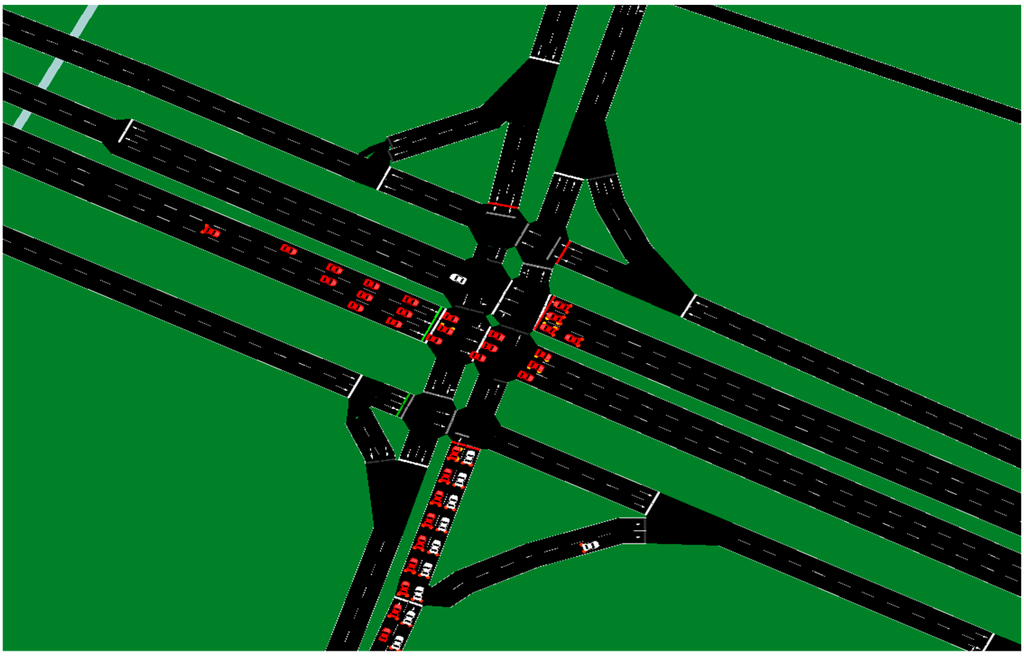
\includegraphics{sumo-simulator}
	\caption[Captura de pantalla del simulador \gls{sumo}]{Captura de pantalla del simulador \gls{sumo}. Además de software de simulación propiamente dicho, \gls{sumo} provee de una interfaz gráfica que permite una visualización general, de zonas y de elementos en concreto a la vez que permite la variación de configuración de la simulación durante el desarrollo de la misma.}
	\label{fig:sumo-simulator}
\end{figure}

\gls{sumo}\index{SUMO} es un entorno de micro-simulación\index{micro-simulación} licenciado bajo la \gls{gpl}\index{GNU General Public License} versión $3$.$0$ y desarrollado por el instituto de sistemas de transporte del Centro Aeroespacial Alemán. Implementa un modelo discreto en el tiempo y continuo en el espacio.

Además de simulación clásica, incorpora una interfaz gráfica (se puede ver una captura de la vista gráfica en la figura~\ref{fig:sumo-simulator}) donde se puede ver el comportamiento de cada vehículo durante la simulación. Es interesante para obtener de un vistazo información acerca del funcionamiento del modelo en concreto a controlar. Otras de las características que el simulador ofrece son las siguientes:

\begin{itemize}
	\item Granularidad micro y meso.
	\item Multimodalidad permitiendo modelar no sólo tráfico de vehículos sino de peatones, bicicletas, trenes e incluso de barcos.
	\item Simulación con y sin colisiones de vehículos.
	\item Diferentes tipologías de vehículos y de carreteras, cada una con diferentes carriles y éstas con diferentes subdivisiones de subcarriles (diseño conceptual para permitir modelar comportamientos en vehículos como motocicletas y similares).
\end{itemize}

Al estar licenciado bajo la licencia \gls{gpl}\index{GNU General Public License}, su distribución implica a su vez la distribución de su código fuente. Esto permite la modificación de su comportamiento y el desarrollo de nuevos modelos integrados dentro del simulador. Sin embargo nosotros no haremos uso de esta característica, sino que usaremos \gls{sumo}\index{SUMO} como aplicación servidor y el módulo \gls{traci}\index{TraCI} como aplicación cliente desde donde gestionar todos los aspectos de la simulación.

\subsection{Modelos de conductor}

\gls{sumo}\index{SUMO} usa como modelo por defecto de \textit{\gls{car-following}\index{car-following}} el modelo de Stefan Krauß \cite{krauss1998microscopic}, debido a su simplicidad y su velocidad de ejecución. Como modelo de cambio de carril, usa el modelo de Gipps \cite{Gipps1986}.

Además de estos modelos, se encuentran para seleccionar otros modelos longitudinales y laterales, como por ejemplo el \gls{idm}, el modelo de tres fases de Kerner \cite{kerner2008testbed} y el modelo de Wiedemann \cite{wiedemann1974simulation}.

\paragraph{Modelo longitudinal de Krauß}

Se trata de un modelo estocástico basado en un esquema discreto de \textit{estímulo}$\rightarrow$\textit{respuesta} donde la velocidad en cada paso de tiempo se calcula de la forma que expresa la ecuación~\ref{eq:krauss-model}.

\begin{equation}
	v_{t+1} = max(0, v_{t+1}^{d} - X \epsilon a_t)
	\label{eq:krauss-model}
\end{equation}

En ésta, la velocidad deseada $v_{t+1}$ se calcula a partir de la velocidad deseada $v_{t+1}^{d}$ menos un valor que depende de la \textit{imperfección} del conductor $\epsilon$ (cuanto mayor es, más errático es el movimiento), la aceleración $a$ del vehículo y un valor aleatorio $X \sim \mathcal{N}(0, 1)$.

El valor de la velocidad deseada $v_{t+1}^{d}$ se calcula de acuerdo a la ecuación~\ref{eq:krauss-model-desired-speed}.

\begin{equation}
	v_{t+1}^{d} = min(v_{t+1}^{s}, v_t + a, v_{max})
	\label{eq:krauss-model-desired-speed}
\end{equation}

Donde $v_{t+1}^{s}$ es la velocidad segura en función de la diferencia de velocidad con el vehículo delantero y $v_{max}$ la velocidad máxima permitida en la vía.

Por último, para el cálculo de la velocidad segura $v_{t+1}^{s}$ se usa la ecuación~\ref{eq:krauss-model-safe-speed}.

\begin{equation}
	v_{t+1}^{s} = v_{t-1}^l + \frac{d - v_{t-1}^l \tau}{\frac{v_{t-1}}{2b + \tau}}
	\label{eq:krauss-model-safe-speed}
\end{equation}

En ésta, $b$ es la deceleración del vehículo, $d$ la distancia de separación entre el vehículo actual y el líder, $v_{t-1}$ y $v_{t-1}^l$ la velocidad en el instante ${t-1}$ de los vehículos actual y líder respectivamente, y $\tau \in [0, \inf)]$ el tiempo de reacción del modelo.

\paragraph{Modelo de cambio de carril de Gipps}

El cálculo de cambio de carril de Gipps \cite{Gipps1986} se basa en la ejecución de la siguiente secuencia de acciones:

\begin{enumerate}
	\item ¿Es \textbf{necesario} cambiar de carril?
	\item ¿Es \textbf{deseable} cambiar de carril?
	\item ¿Es \textbf{posible} cambiar de carril?
\end{enumerate}

El artículo dedicado al modelo de control lateral es muy extenso como para reproducir el contenido aquí. Basta mencionar que cada una de las acciones se basa en un cálculo sobre un indicador principal: la \textbf{distancia} a finales de carril o a desvíos en intersecciones (\textbf{necesidad} de cambio de carril), la diferencia entre la \textbf{velocidad} deseada y velocidad posible (\textbf{deseo} de cambio de carril) y \textbf{hueco} existente en carriles laterales (\textbf{posibilidad} de cambio de carril).

Un detalle que hay que tener en cuenta es el siguiente: el modelo de cambio de carril usado en \gls{sumo}\index{SUMO} es el de Krauß \cite{krauss1998microscopic}, pero el modelo de cambio de carril se basa en las ecuaciones de su propio modelo longitudinal \cite{Gipps1981}. Sin embargo, en el propio artículo indican que aunque base sus ecuaciones en el modelo anterior, la única imposición sobre el modelo longitudinal es que el incremento de velocidad esté acotado superiormente, restricción que se cumple en el modelo de Krauß (ver ecuación{\ref{eq:krauss-model-desired-speed}).

\subsection{La interfaz \gls{traci}\index{TraCI}}

\gls{traci}\index{TraCI} \cite{Wegener2008} es tanto el nombre del protocolo de comunicación expuesto por \gls{sumo}\index{SUMO} en su versión servidor como el nombre de la librería escrita en \gls{python}\index{Python} para interactuar con el mismo. Como protocolo, la interacción a través de cliente/servidor comienza especificando a \gls{sumo}\index{SUMO} que se desea trabajar de este modo. En ese momento, \gls{sumo}\index{SUMO} se inicializa en modo servidor dejando abierto un puerto TCP para la conexión del cliente (figura~\ref{fig:traci-messages} \subref{fig:traci-messages-a}).

\begin{figure}
	\centering
	\subfloat[Conexión.\label{fig:traci-messages-a}]{
		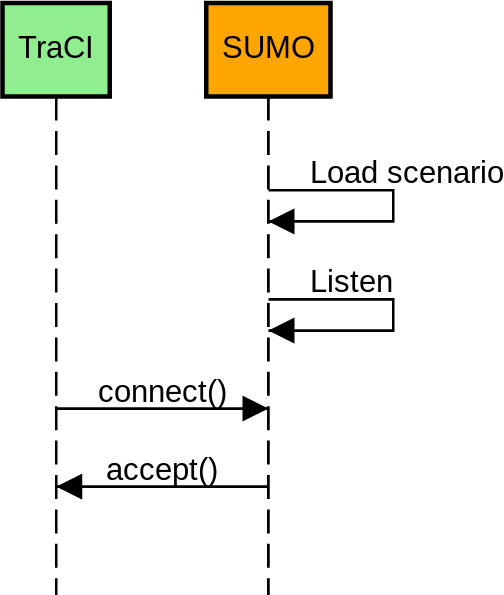
\includegraphics[width=0.31\linewidth]{sequence-diagram-traci-sumo-connect}
	}
	\subfloat[Envío de mensajes.\label{fig:traci-messages-b}]{
		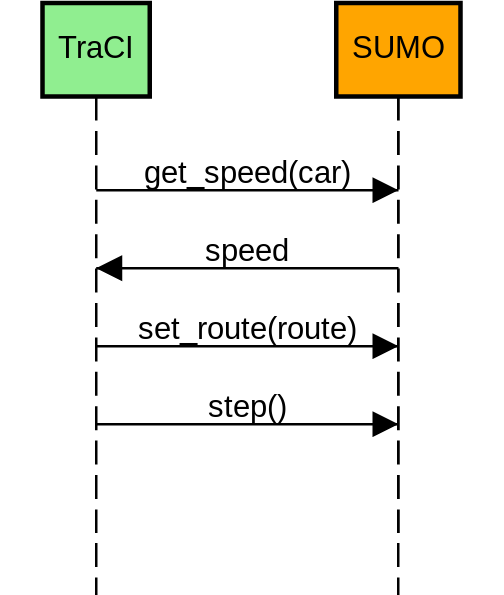
\includegraphics[width=0.31\linewidth]{sequence-diagram-traci-sumo-some-messages}
	}
	\subfloat[Desconexión.\label{fig:traci-messages-c}]{
		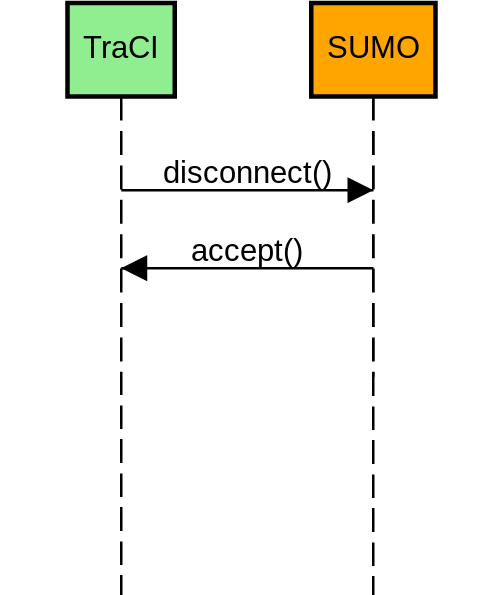
\includegraphics[width=0.31\linewidth]{sequence-diagram-traci-sumo-disconnect}
	}
	\caption[Ejemplo de forma de envío de mensajes a través de TraCI]{Ejemplo de forma de envío de mensajes a través de TraCI. \gls{sumo} ofrece la posibilidad de interactuar con la simulación desde cualquier aplicación a través del uso del protocolo \gls{traci}. En la figura podemos ver, de izquierda a derecha, ejemplos de comunicación a través de la interfaz como el \textit{handshake} o inicialización, mensajes de obtención de información y modificación de la misma más una solicitud de avance de paso en la simulación y una señal de finalización de simulación y desconexión.}
	\label{fig:traci-messages}
\end{figure}

Una vez el servidor se encuentra en ese estado, el cliente se conecta enviando una señal de conexión indicando que él se encargará de controlar la simulación. Desde ese momento y hasta que el cliente no envíe una señal de desconexión (figura~\ref{fig:traci-messages} \subref{fig:traci-messages-c}), el cliente podrá enviar y recibir todos los mensajes que desee para capturar información y modificar los detalles de la simulación, incluido el mensaje \textit{step}, que es el encargado de avanzar un paso en la simulación (figura~\ref{fig:traci-messages} \subref{fig:traci-messages-b}).

Como librería, \gls{traci}\index{TraCI} es un módulo desarrollado en \gls{python}\index{Python} $2$.$7$. Aunque es posible trabajar directamentea través de sockets, una librería abstrae todos los detalles dando una interfaz de trabajo más clara y sencilla.

Aunque no se usará en esta tesis, existe una implementación que provee de una capa de abstracción por encima: \gls{traas}\index{TraaS}\sidenote{\url{http://traas.sourceforge.net/cms/}.}. Esta plataforma ofrece toda la funcionalidad de \gls{traci}\index{TraCI} como SaaS, proporcionando una interfaz de servicios Web bajo protocolo SOAP para abstraer el protocolo en mensajes HTTP (figura~\ref{fig:traas}).

\begin{figure}
	\centering
	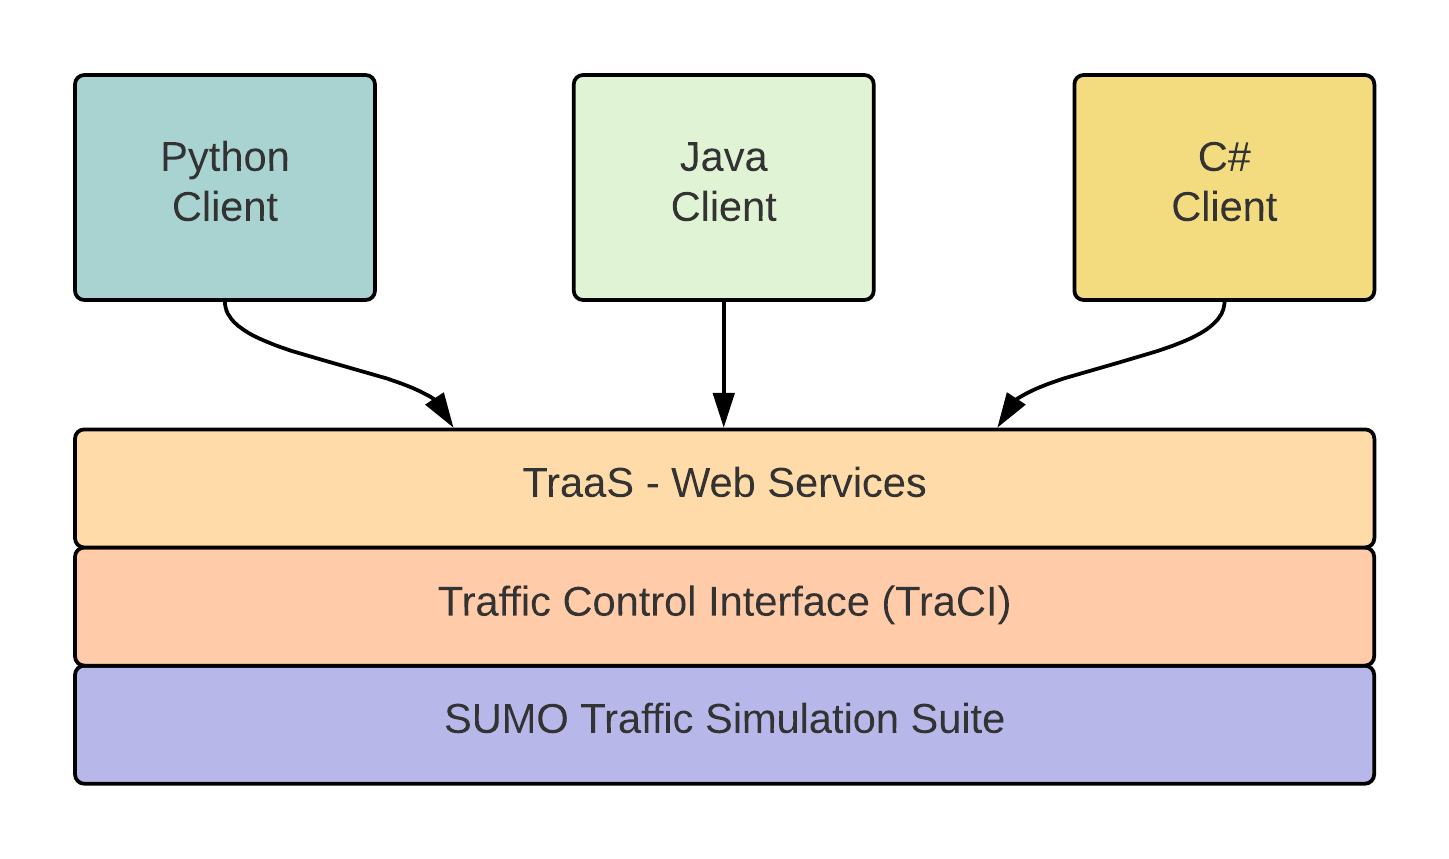
\includegraphics[width=.7\textwidth]{traas-architecture}
	\caption[Arquitectura de la plataforma \gls{traas}]{Arquitectura de la plataforma \gls{traas}. La plataforma se conecta como cliente a \gls{sumo} y ofrece un \glsentryshort{api} basado en \glsentryshort{soap} de mensajes que traduce en mensajes del protocolo \gls{traci}, lo que independiza completamente la elección de lenguaje de programación a la vez que abstrae los detalles del protocolo de comunicación.}
	\label{fig:traas}
\end{figure}
